\Chapter{Mérések}

\section{Numerikus integrálás}

\subsection{Trapézszabály}
\subsubsection{Rövid matematikai bevezetés}
A trapézszabály határozott integrálok meghatározására alkalmas közelítő módszer, amely egy adott intervallumba eső függvénygörbe alatti területet a függvénygörbe (vég)pontjaira illesztett trapézzal közelíti. Azaz, ha a és b számok az intervallum végpontjai, akkor:
\[ \int_{a}^{b} f(x) dx \approx (b-a) * \frac{f(a) + f(b)}{2} \]
\subsubsection{C nyelvű referencia-implementáció}
\cppstyle{\begin{lstlisting}[language=c++]
float trapedozial_rule(float a, float b, int n) {
    float x;
    float s;
    float h;

    h = (b-a) / n;
    x = a;
    b = 0.0;

    for (int i = 0; i < n; i++) {
        x += h;
        s += parameter_function(x);
    }
    return 0.5 * (parameter_function(a) + 2.0 * s + parameter_function(b) );
}
\end{lstlisting}}
\subsubsection{Az algoritmus egy implementációja Rustban}
\begin{lstlisting}[language=Rust, style=boxed]
fn trapedozial_rule(a: f32, b: f32, n: i32) -> f32 {
  let mut _x: f32;
  let mut _s: f32;
  let h: f32;
  
  h = (b-a) / (n as f32);
  _x = a;
  _s = 0.0;
  for _i in 1..n {
	  _x += h;
	  _s += parameter_function(_x);
  }
  return 0.5 * (parameter_function(a) + 2.0 * _s + parameter_function(b) );
}
\end{lstlisting}

\subsubsection{Futtatások eredményei}

\subsection{Iteratív trapézszabály}
\subsubsection{Rövid matematikai bevezetés}
Az iteratív trapézszabály a trapézszabályra épül. Lényege, hogy a függvénygörbe alatti területre illesztett trapézok számát iteratívan növeli, így minden iterációban egyre jobb közelítést ad. A számítógép implementációk esetén ez a finomítási folyamat akkor áll meg, amikor az elmúlt iterációban nem változott "sokat" a közelítés értéke.
\subsubsection{C nyelvű referencia-implementáció}
\cppstyle{\begin{lstlisting}[language=c++]
float q_trapedozial_rule(float a, float b) {
    const int J_MAX = 20;
    const float EPS = 0.00001;

    float s = 0.0;
    float olds;

    olds = -0.00000000000000000000000000001;
    for (int j = 0; j < J_MAX; j++) {
        s = trapedozial_rule(a, b, j);
        if (j < 5) {
            if (abs(s-olds) < EPS * abs(olds) ) {
                if ( (s == 0.0) && (olds == 0.0) ) {
                    return s;
                }
            }
        }
    }
    return s;
}
\end{lstlisting}}
\subsubsection{Az algoritmus egy implementációja Rustban}
\begin{lstlisting}[language=Rust]
fn q_trapedozial_rule(a: f32, b: f32) -> f32 {
  const J_MAX: i32 = 20;
  const EPS: f32 =  0.00001;
  
  let mut s: f32 = 0.0;
  let olds: f32;
  
  olds = -0.00000000000000000000000000001;
  println!("{}", olds);
  for j in 0..J_MAX {
	  s = trapedozial_rule(a, b, j);
	  if j > 5 {
		  if (s-olds).abs() < EPS * olds.abs() {
			  if s == 0.0 && olds == 0.0 {
				  return s;
			  }
		  }
	  }
  }
  return s;
}
\end{lstlisting}

\subsubsection{Futtatások eredményei}

\subsection{Iteratív Simpson-módszer}
\subsubsection{Rövid matematikai bevezetés}
A Simpson-módszer a trapézszabályon alapul úgy, hogy a részintervallumok végpontjaihoz súlyokat rendel.Az iteratív Simpson-módszer a Simpson-módszerre alapul, az iteratív trapézszabályhoz hasonlóan finomítja egyre jobban a közelítést minden iterációban.
\subsubsection{C nyelvű referencia-implementáció}
\cppstyle{\begin{lstlisting}[language=c++]
float q_simpsons_rule(float a, float b) {
    const int J_MAX = 20;
    const float EPS = 0.00001;

    float s = 0.0;
    float st;
    float ost;
    float os;

    os = -0.00000000000000000000000000001;
    ost = os;

    for (int j = 0; j < J_MAX; j++) {
        st = trapedozial_rule(a, b, j);
        s = (4.0 * st - ost) / 3.0;
        if (j < 5) {
            if (abs(s-os) < EPS * abs(os) || (s == 0.0 && os == 0.0) ) {
                return s;
            }
        }
        os = s;
        ost = st;
    }
    return s;
}
\end{lstlisting}}
\subsubsection{Az algoritmus egy implementációja Rustban}
\begin{lstlisting}[language=Rust]
fn q_simpsons_rule(a: f32, b: f32) -> f32 {
  const J_MAX: i32 = 20;
  const EPS: f32 = 0.000001;
	  
  let mut s: f32 = 0.0;
  let mut st: f32;
  let mut ost: f32;
  let mut os: f32;
  
  os = -0.00000000000000000000000000001;
  ost = os;
  
  for j in 0..J_MAX {
	  st = trapedozial_rule(a, b, j);
	  s = (4.0 * st - ost) / 3.0;
	  if j < 5 {
		  if (s-os).abs() < EPS * os.abs() || (s == 0.0 && os == 0.0) {
			  return s;
		  }
	  }
	  os = s;
	  ost = st;
  }
  return s;
}
\end{lstlisting}
\subsubsection{Futtatások eredményei}

\subsection{Gauss-Legendre-módszer}
\subsubsection{Rövid matematikai bevezetés}
\subsubsection{C nyelvű referencia-implementáció}
\cppstyle{\begin{lstlisting}[language=c++]
float q_gauss_legendre(float a, float b) {
    float xr;
    float xm;
    float dx;
    float s;

    const float[6] X = [0.0, 0.1488743389, 0.4333953941, 0.6794095682,
        0.8650633666, 0.9739065285];
    const float[6] Y = [0.0, 0.2955242247, 0.2692667193, 0.2190863625,
        0.1494513491, 0.0666713443];

    xm = 0.5 * (b + a);
    xr = 0.5 * (b - a);

    s = 0.0;

    for (j = 0; j < 5; j++) {
        dx = xr * X[j];
        s += W[j] * parameter_function(xm + dx) + parameter_function(xm - dx);
    }

    float result = s * xr;
    return result;
}
\end{lstlisting}}
\subsubsection{Az algoritmus egy implementációja Rustban}
\begin{lstlisting}[language=Rust]
fn q_gauss_legendre(a: f32, b: f32) -> f32 {
  let xr: f32;
  let xm: f32;
  let mut dx: f32;
  let mut s: f32;
  
  const X: [f32; 6] = [0.0, 0.1488743389, 0.4333953941, 0.6794095682,
      0.8650633666, 0.9739065285];
  const W: [f32; 6] = [0.0, 0.2955242247, 0.2692667193, 0.2190863625,
      0.1494513491, 0.0666713443];
  
  xm = 0.5 * (b + a);
  xr = 0.5 * (b - a);
  
  s = 0.0;
  
  for j in 0..5 {
	  dx = xr * X[j];
	  s += W[j] * parameter_function(xm + dx) + parameter_function(xm - dx);
  }
  
  let result: f32 = s * xr;
  return result;
}  
\end{lstlisting}
\subsubsection{Futtatások eredményei}

\section{Rendezés}

\subsection{Kupac-rendezés}
\subsubsection{Rövid matematikai bevezetés}
\subsubsection{C nyelvű referencia-implementáció}
\cppstyle{\begin{lstlisting}[language=c++]
void heapify(Vec *a, unsigned n, unsigned i) {
    unsigned largest = i;
    unsigned l = 2 * i + 1;
    unsigned r = 2 * i + 2;

    if ( (r < n) && (a->elements[i] < a->elements[l]) ) {
        largest = l;
    }

    if ( (r < n) && (a->elements[largest] < a->elements[r]) ) {
        largest = r;
    }

    if (largest != i) {
        SWAP(float, a->elements[largest], a->elements[i]);

        heapify(a, n, largest);
    }
}

void heapsort(unsigned n, Vec *a) {
    unsigned i = n;
    while (i > 0) {
        heapify(a, n, i);
        i -= 1;
    }

    i = n - 1;
    while (i > 0) {
        SWAP(float, a->elements[0], a->elements[i]);
        heapify(a, i ,0);
        i -= 1;
    }
}
\end{lstlisting}}
\subsubsection{Az algoritmus egy implementációja Rustban}
\begin{lstlisting}[language=Rust]
fn heapify(a: &mut Vec<f32>, n: usize, i: usize) {
	let mut largest: usize = i;
	let l = 2 * i + 1;
	let r = 2 * i + 2;
	
	if r < n && a[i] < a[l] {
		largest = l;
	}
	
	if r < n && a[largest] < a[r] {
		largest = r;
	}
	
	if largest != i {
		a.swap(largest, i);
		
		heapify(a, n, largest);
	}
}

pub fn heapsort(n: usize, a: &mut Vec<f32>) {
	let mut i: usize = n;
	while i > 0 {
		heapify(a, n, i);
		i -= 1;
	}

	i = n - 1;
	while i > 0 {
		a.swap(0, i);
		heapify(a, i, 0);
		i -= 1;
	}
}
\end{lstlisting}
\subsubsection{Futtatások eredményei}
Kupac-rendezés futási ideje

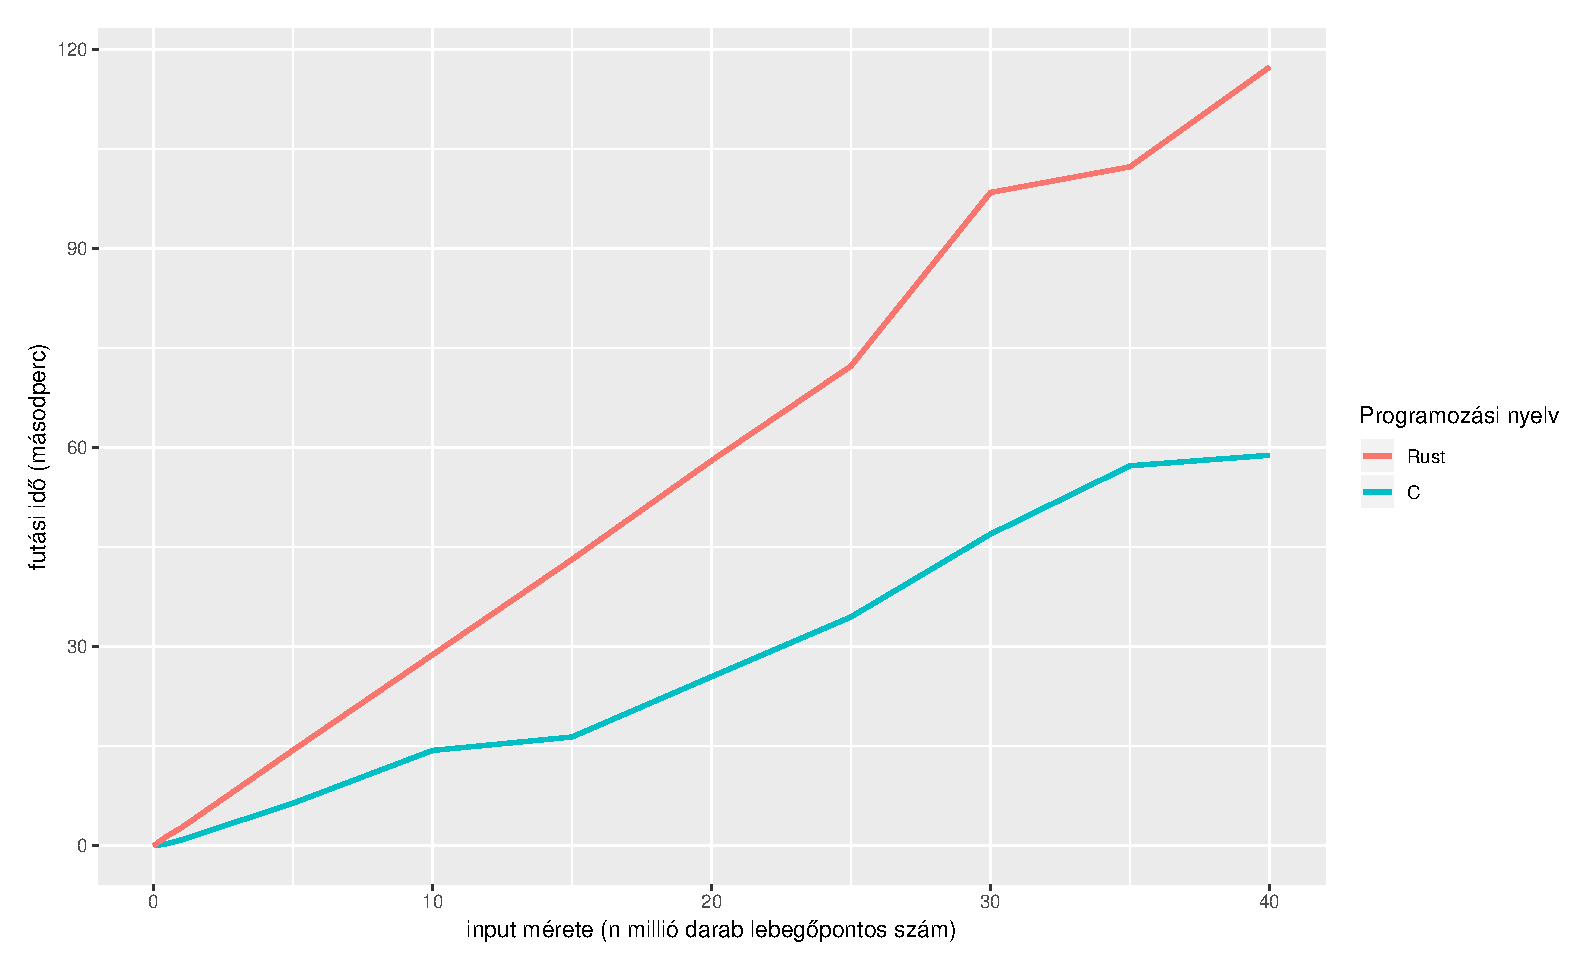
\includegraphics[width=15.5cm]{kepek/heap_run.eps}
Látható, hogy a kupac-rendezés módszerét tekintve a Rust nyelvű implementáció lassabb, mint a C-s megfelelője.

Kupac-rendezés maximális memóriafoglalása

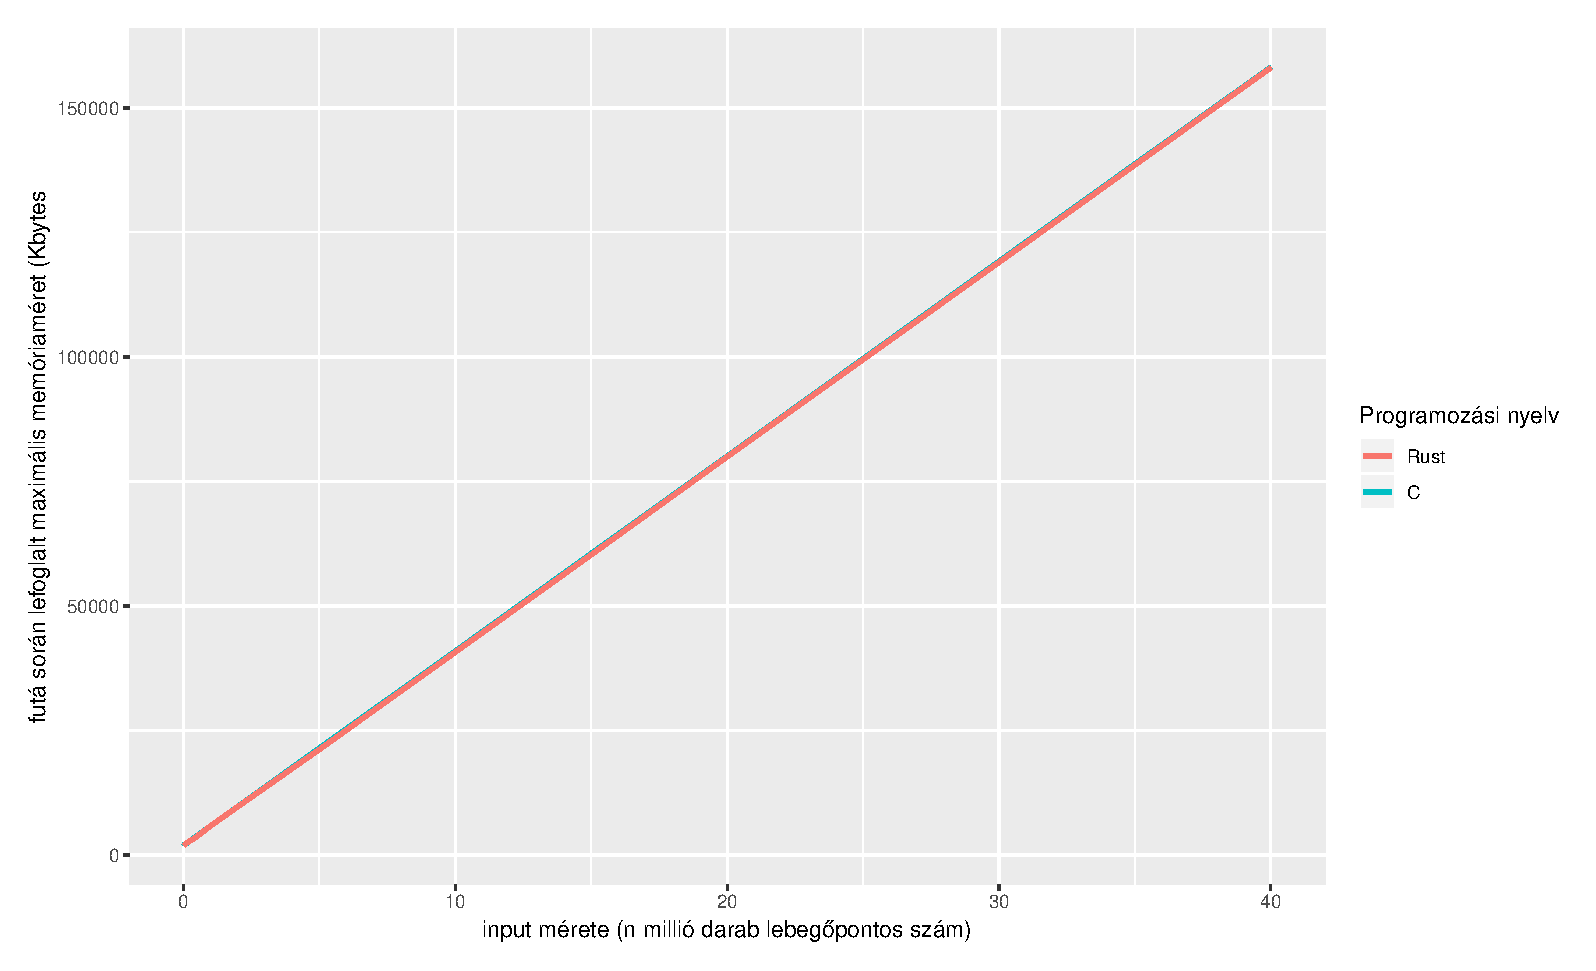
\includegraphics[width=15.5cm]{kepek/heap_memory.eps}
A Rust és C nyelven elkészített implementációk között a maximális memóriafoglalást tekintve nincsenek jelentős eltérések.

\subsection{Shell-rendezés}
\subsubsection{Rövid matematikai bevezetés}
\subsubsection{C nyelvű referencia-implementáció}
\cppstyle{\begin{lstlisting}[language=c++]
void shell_sort(unsigned n, Vec *a) {
    int gap = (n / 2);
    float temp;
    int j;

    while (gap > 0) {
        for (unsigned i = gap; i < n; i++) {
            temp = a->elements[i];
            
            j = i;
            while ( (j >= gap) && (a->elements[(j-gap)] > temp) ) {
                a->elements[j] = a->elements[(j-gap)];
                j -= gap;
            }
            a->elements[j] = temp;
        }
        gap /= 2;
    }
}
\end{lstlisting}}
\subsubsection{Az algoritmus egy implementációja Rustban}
\begin{lstlisting}[language=Rust]
pub fn shell_sort(n: i32, a: &mut Vec<f32>) {
	let mut gap: i32 =  (n / 2) as i32;
	let mut temp: f32;
	let mut j: i32;
	
	while gap > 0 {
		for i in gap..n {
			temp = a[i as usize];
			
			j = i;
			while j >= gap && a[(j-gap) as usize] > temp {
				a[j as usize] = a[(j-gap) as usize];
				j -= gap;
			}
			a[j as usize] = temp;
		}
		gap /= 2;
	}
}
\end{lstlisting}
\subsubsection{Futtatások eredményei}
Shell-rendezés futási ideje

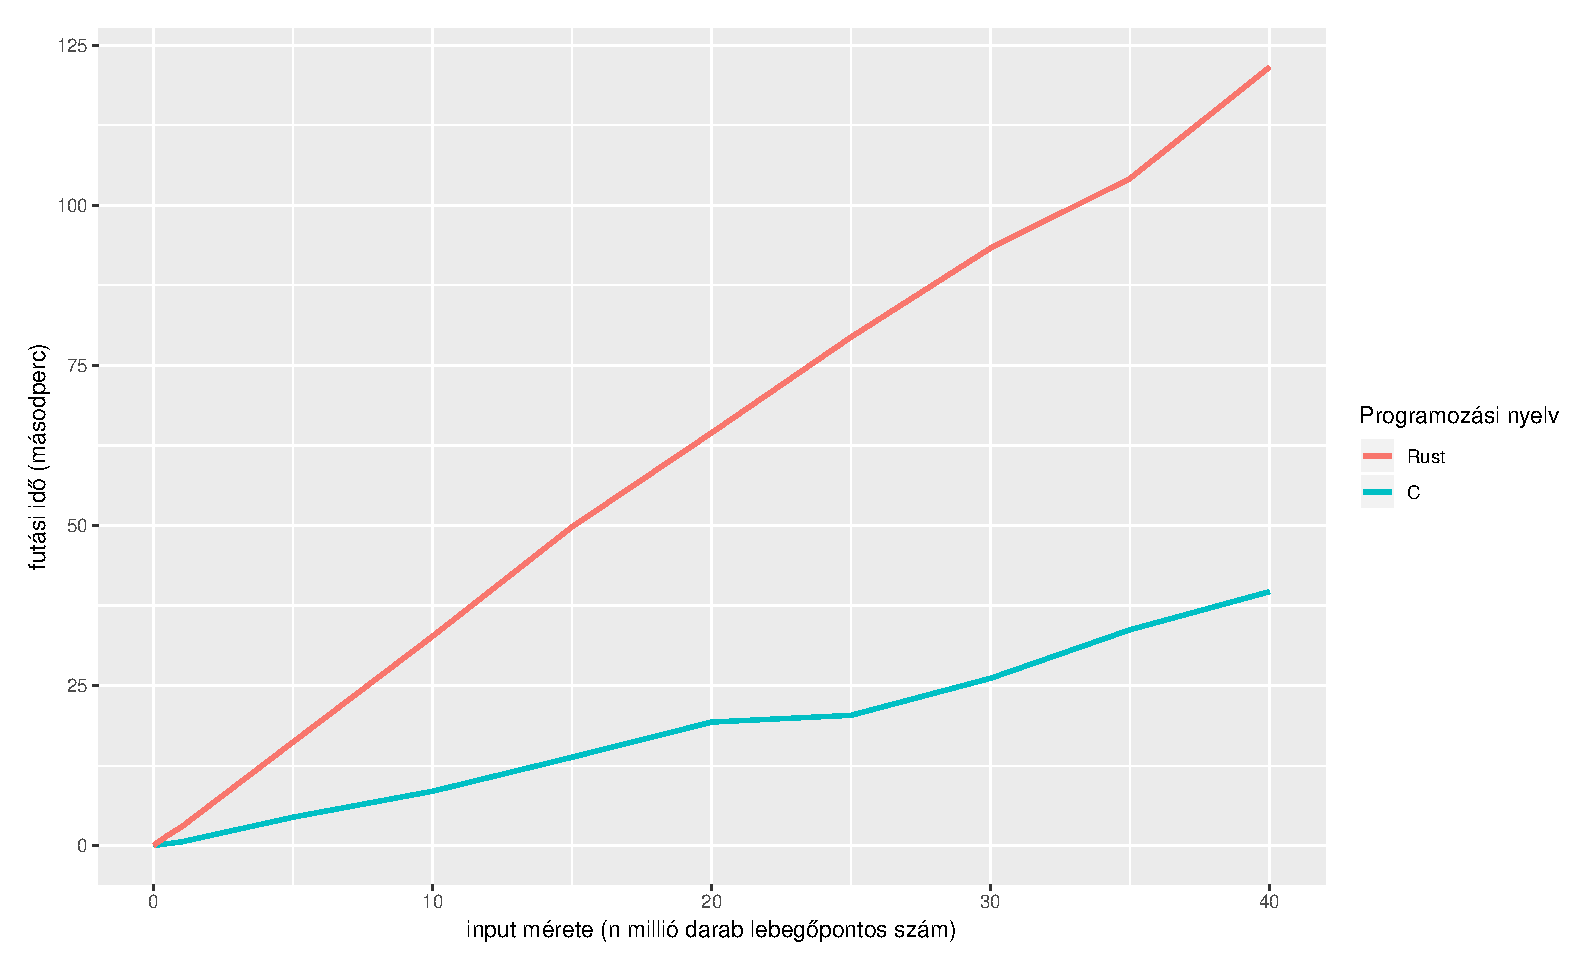
\includegraphics[width=15.5cm]{kepek/shell_run.eps}
Látható, hogy a Shell-rendezés módszerét tekintve a Rust nyelvű implementáció lassabb, mint a C-s megfelelője.

Shell-rendezés maximális memóriafoglalása

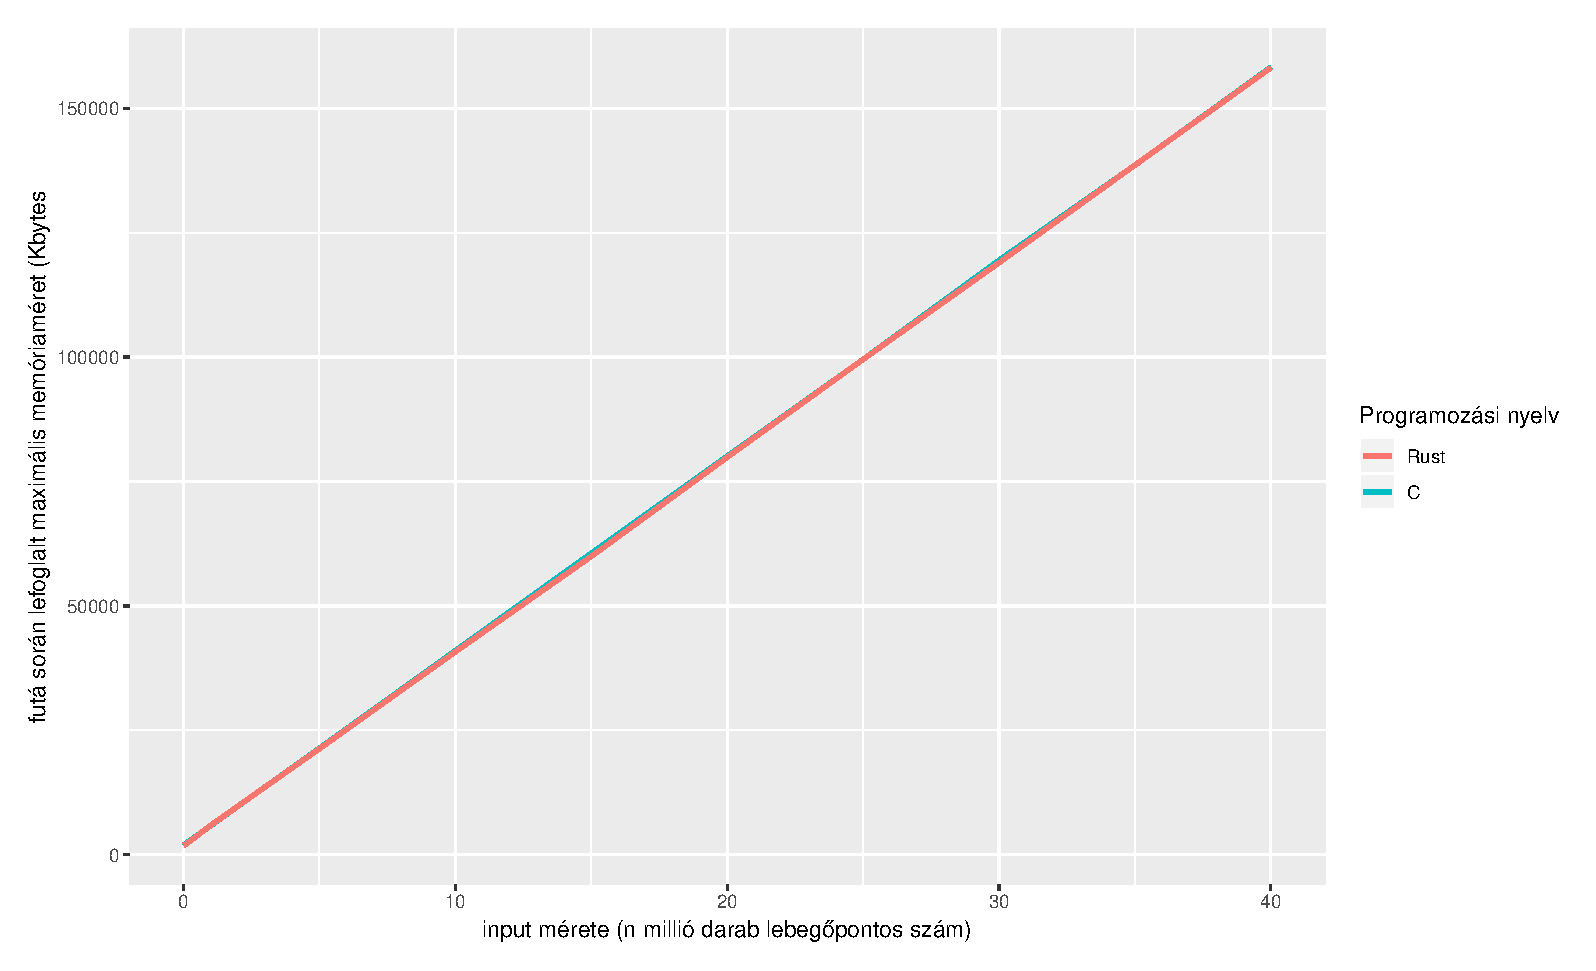
\includegraphics[width=15.5cm]{kepek/shell_memory.eps}
A Rust és C nyelven elkészített implementációk között a maximális memóriafoglalást tekintve nincsenek jelentős eltérések.

\subsection{Gyorsrendezés (Quicksort)}
\subsubsection{Rövid matematikai bevezetés}
\subsubsection{C nyelvű referencia-implementáció}
\cppstyle{\begin{lstlisting}[language=c++]
int partition(int low, int high, Vec *arr) {
    float pivot;

    int mid = (low + high) / 2;
    if (arr->elements[mid] < arr->elements[low]) {
        SWAP(float, arr->elements[low], arr->elements[high]);
    }

    if (arr->elements[high] < arr->elements[low]) {
        SWAP(float, arr->elements[low], arr->elements[high]);
    }

    if (arr->elements[mid] < arr->elements[high]) {
        SWAP(float, arr->elements[mid], arr->elements[high]);
    }

    pivot = arr->elements[high];

    int i;
    int j;

    i = low - 1;
	j = high + 1;

    while (1) {
        while (1) {
            i += 1;
            if (arr->elements[i] >= pivot) {
                break;
            }
        }

        while (1) {
            j -= 1;
            if (arr->elements[j] <= pivot) {
                break;
            }
        }

        if (i >= j) {
            return j;
        }

        SWAP(float, arr->elements[i], arr->elements[j]);
    }
}

void quicksort(int low, int high, Vec *arr) {
    if (low < high) {
        int p = partition(low, high, arr);
        quicksort(low, p, arr);
        quicksort(p+1, high, arr);
    } else {
        return;
    }
}
\end{lstlisting}}
\subsubsection{Az algoritmus egy implementációja Rustban}
\begin{lstlisting}[language=Rust]
pub fn quicksort(low: i32, high: i32, arr: &mut Vec<f32>) {
	if low < high {
		let p: i32 = partition(low, high, arr);
		quicksort(low, p, arr);
		quicksort(p+1, high, arr);
	} else {
		return;
	}
}

fn partition(low: i32, high: i32, arr: &mut Vec<f32>) -> i32 {
	let pivot: f32;

	let mid: i32 = (low + high) / 2;
	if arr[mid as usize] < arr[low as usize] {
		arr.swap(low as usize, high as usize);
	}
	if arr[high as usize] < arr[low as usize] {
		arr.swap(low as usize, high as usize);
	}
	if arr[mid as usize] < arr[high as usize] {
		arr.swap(mid as usize, high as usize);
	}
	pivot = arr[high as usize];

	let mut i: i32;
	let mut j: i32;

	i = low - 1;
	j = high + 1;

	loop {
		loop {
			i += 1;
			if arr[i as usize] >= pivot {
				break;
			}
		}

		loop {
			j -= 1;
			if arr[j as usize] <= pivot {
				break;
			}
		}

		if i >= j {
			return j as i32;
		}

		arr.swap(i as usize, j as usize);
	}
}
\end{lstlisting}
\subsubsection{Futtatások eredményei}
Gyorsrendezés futási ideje

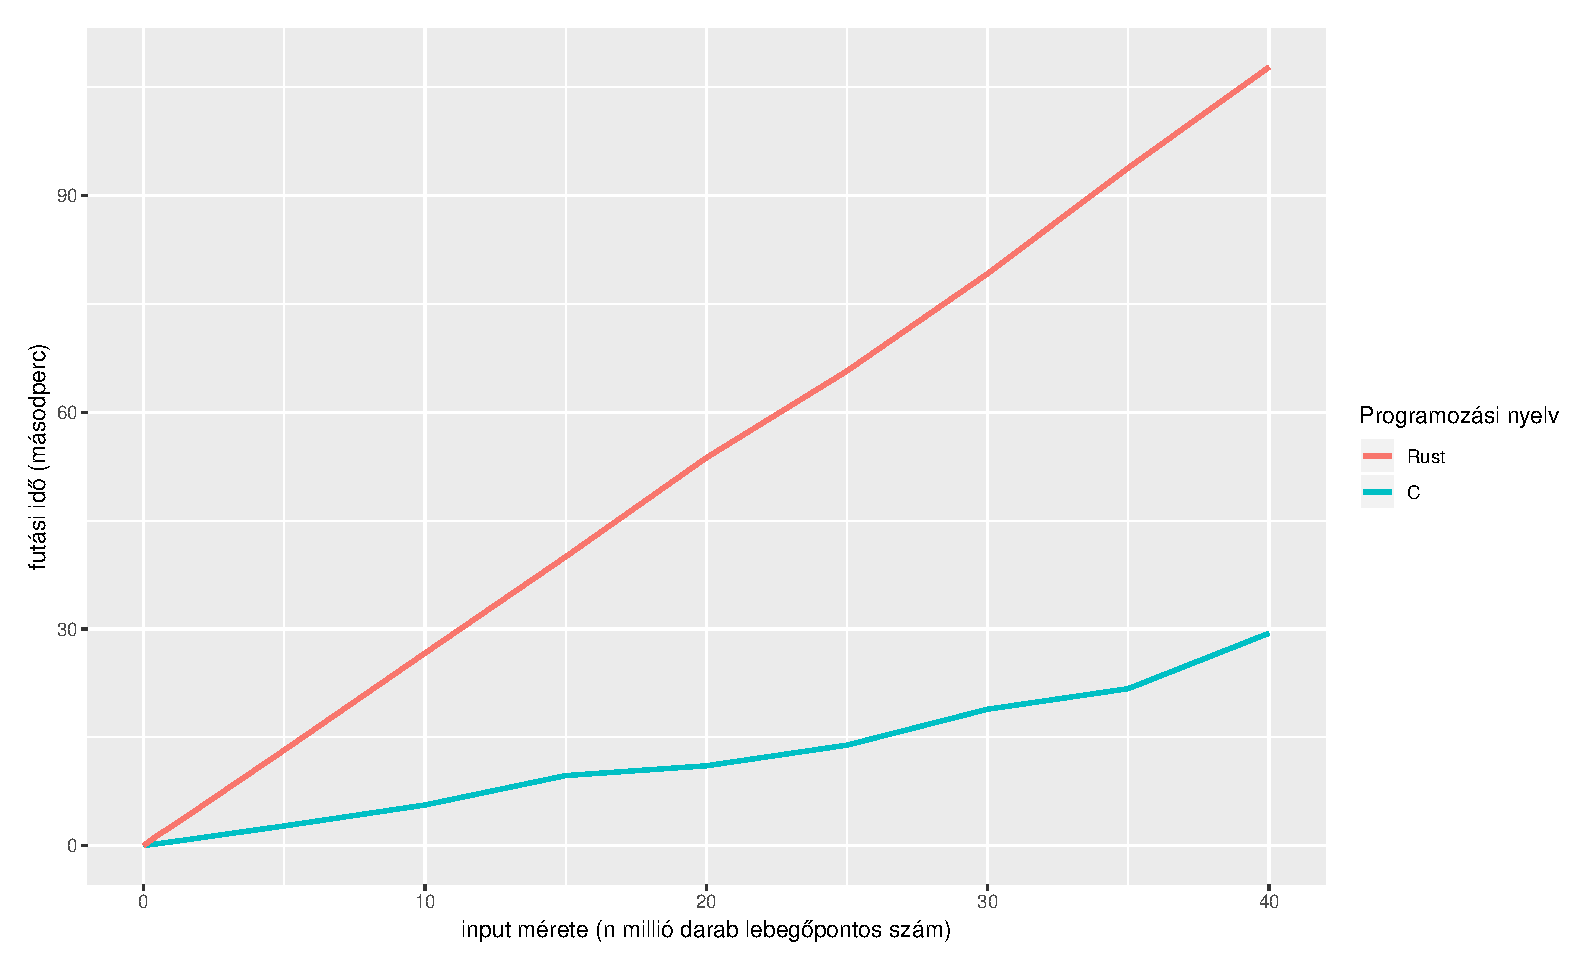
\includegraphics[width=15.5cm]{kepek/quick_run.eps}
Látható, hogy a gyorsrendezés módszerét tekintve a Rust nyelvű implementáció lassabb, mint a C-s megfelelője.

Gyorsrendezés maximális memóriafoglalása

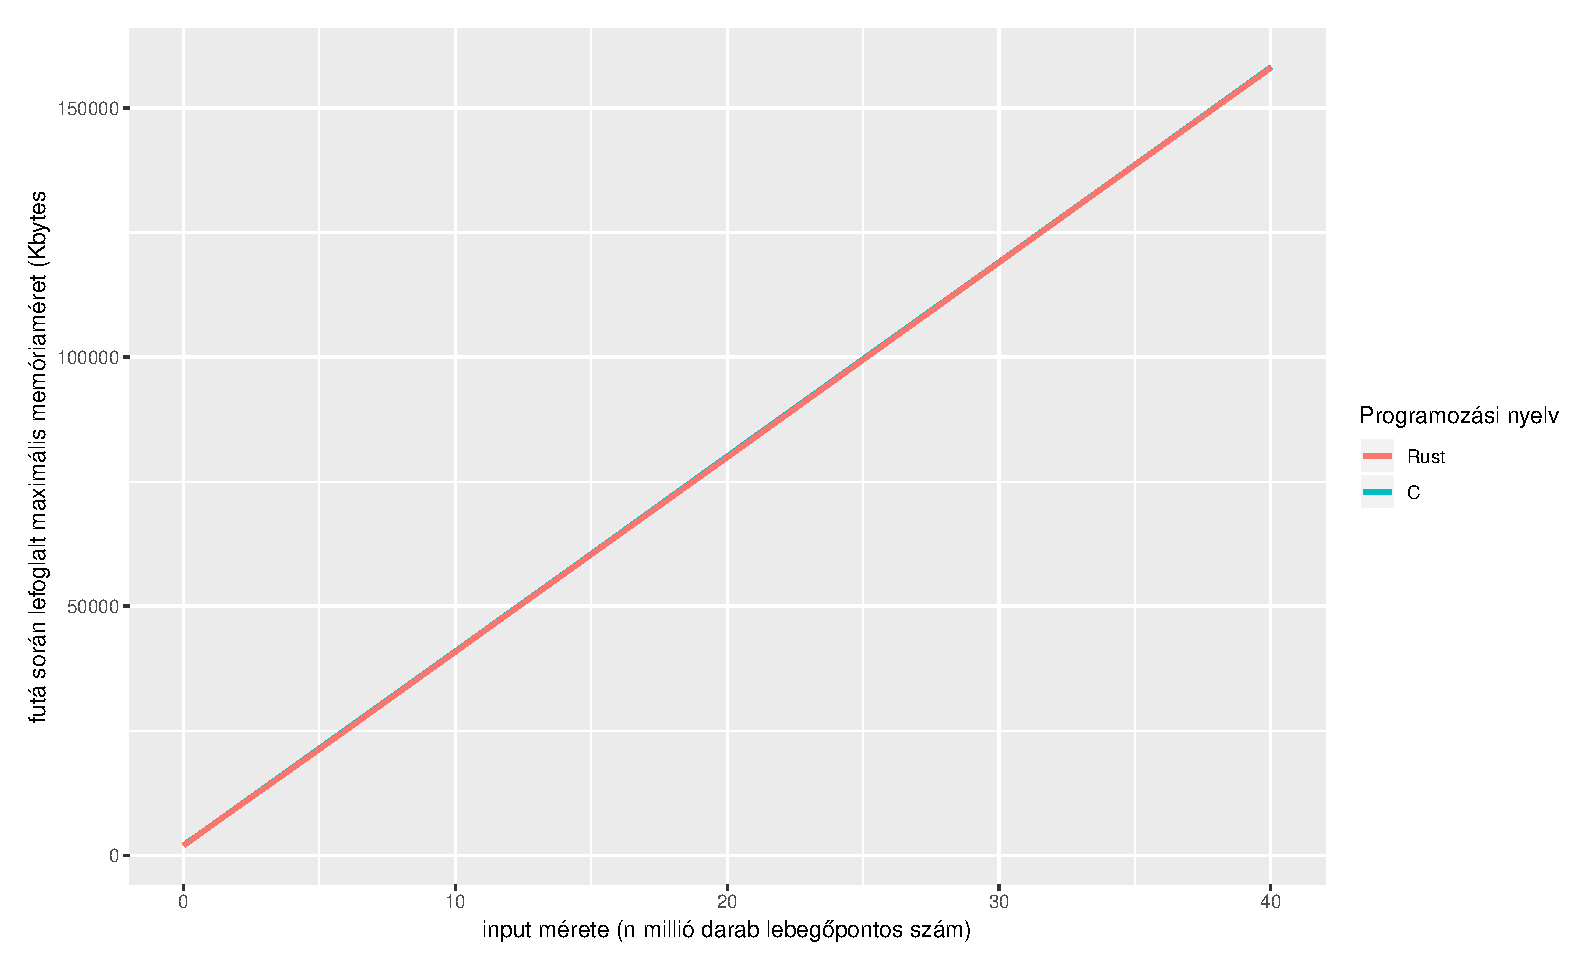
\includegraphics[width=15.5cm]{kepek/quick_memory.eps}
A Rust és C nyelven elkészített implementációk között a maximális memóriafoglalást tekintve nincsenek jelentős eltérések.

\section{Interpoláció}

\subsection{Lineáris interpoláció}
\subsubsection{Rövid matematikai bevezetés}
A lineáris interpoláció két ismert pont közötti összefüggést egyenes arányossággal közelíti. Az ismert pontok által meghatározott egyenesen lévő pontnak így elég az egyik koordinátáját ismerni a másik koordinátájának kiszámításához.
\[ y_n = \frac{x_n - x_1}{x_2 - x_1} * (y_2 - y_1) + y_1 \]
Ahol $x_1 \neq x_2$.
\subsubsection{C nyelvű referencia-implementáció}
\cppstyle{\begin{lstlisting}[language=c++]
float linear_interpolation(float x1, float y1, float x0, float y0, float x) {
    float delta;
    delta = x1 - x0;
    float y;

    if (delta == 0.0) {
        y = y0;
    } else {
        y = y0 + ( (x - x0) / delta) * y1;
    }

    return y;
}
\end{lstlisting}}
\subsubsection{Az algoritmus egy implementációja Rustban}
\begin{lstlisting}[language=Rust]
fn linear_interpolation(x1: f32, y1: f32, x0: f32, y0: f32, x: f32) -> f32 {
  let delta: f32;
  delta = x1 - x0;
  let y;

  if delta == 0.0 {
      y = y0;
  } else {
      y = y0 + ( (x - x0) / delta) * y1;
  }

  return y;
}
\end{lstlisting}
\subsubsection{Futtatások eredményei}
Lineáris interpoláció futási ideje

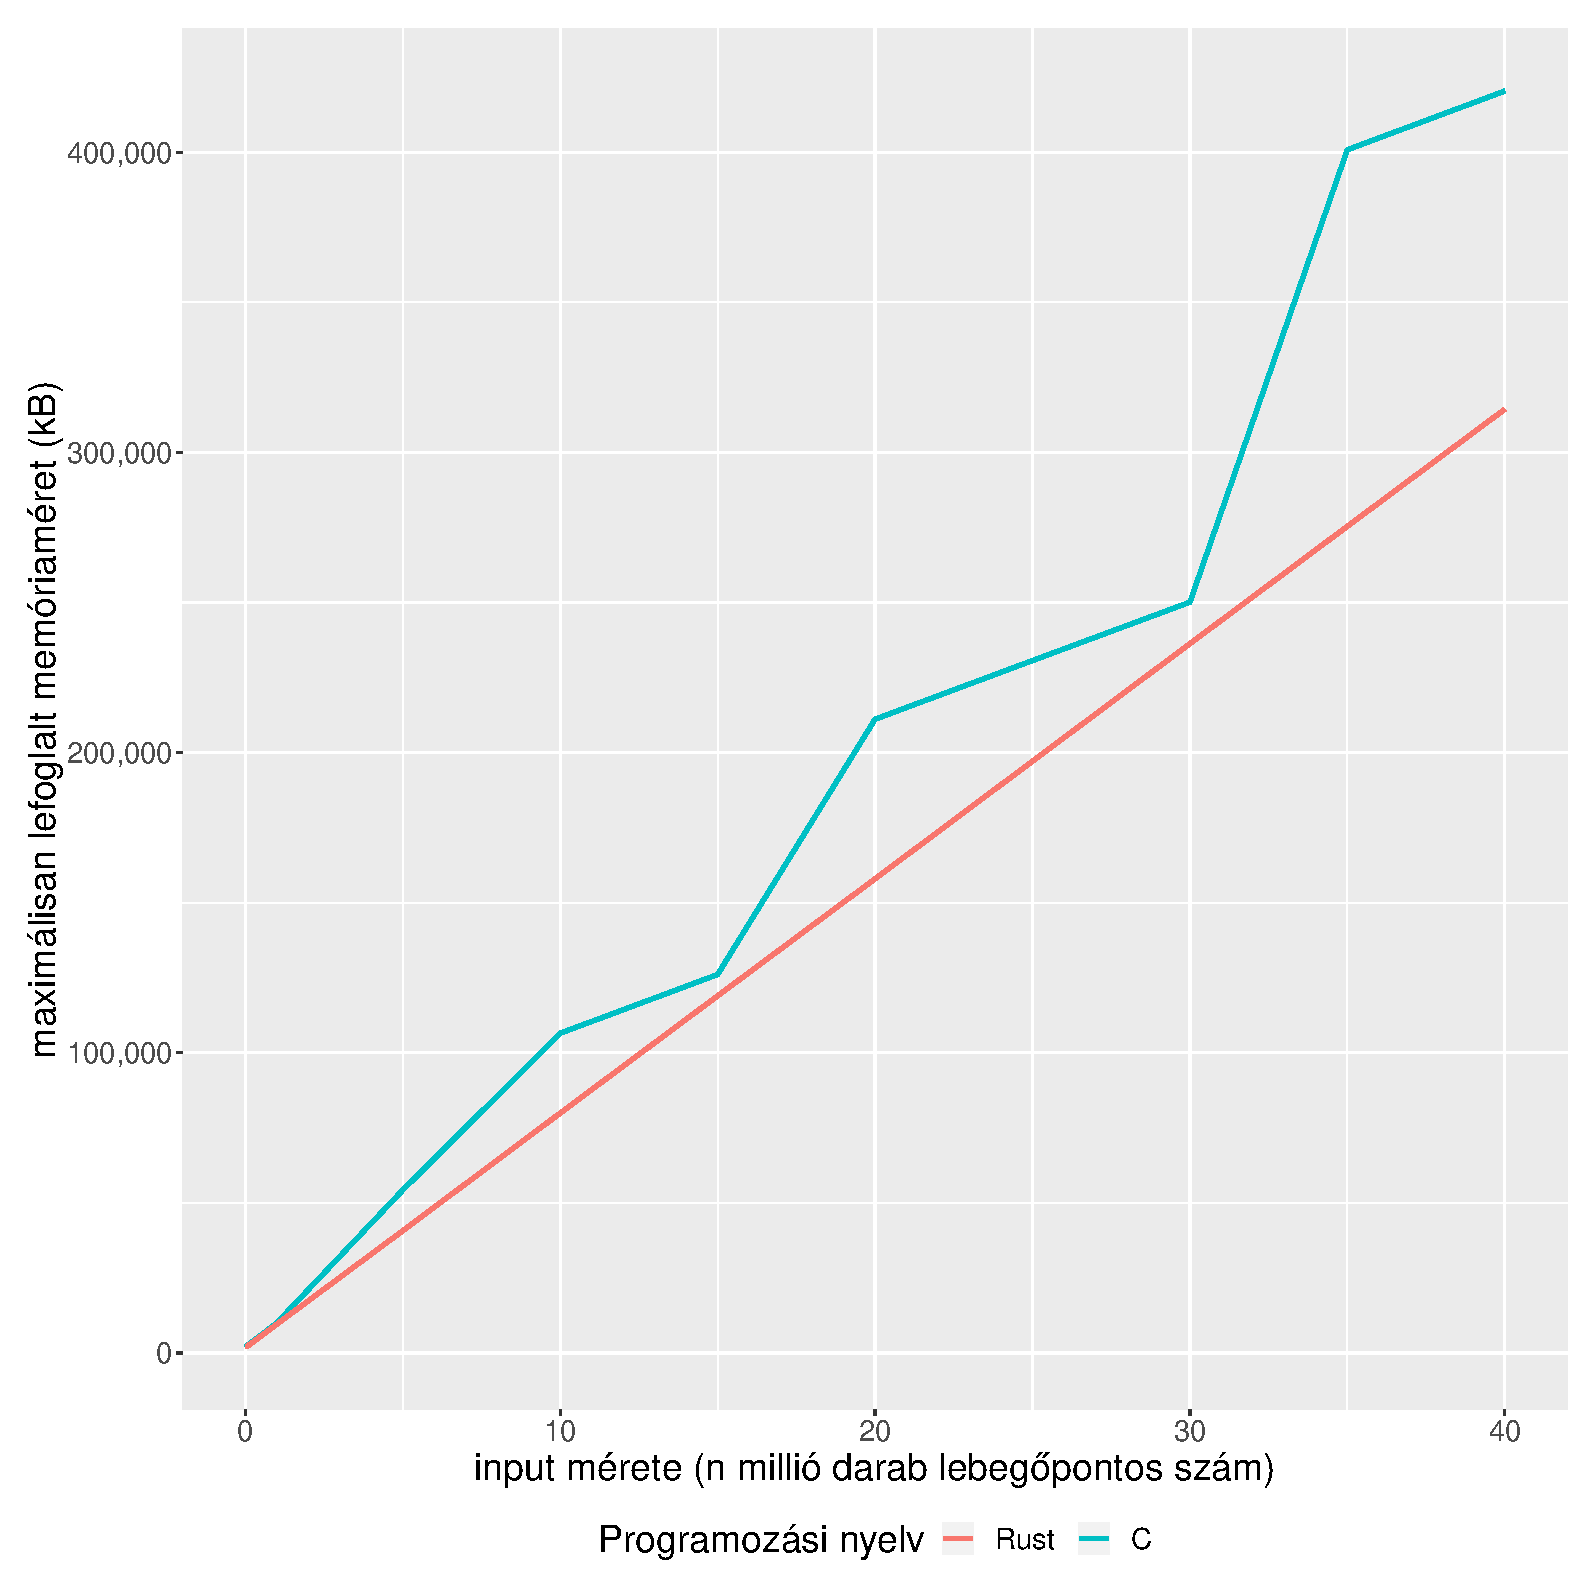
\includegraphics[width=15.5cm]{kepek/linear_interpolation_memory.eps}
Látható, hogy a lineáris interpoláció módszerét tekintve a Rust nyelvű implementáció lassabb, mint a C-s megfelelője.

Lineáris interpoláció maximális memóriafoglalása

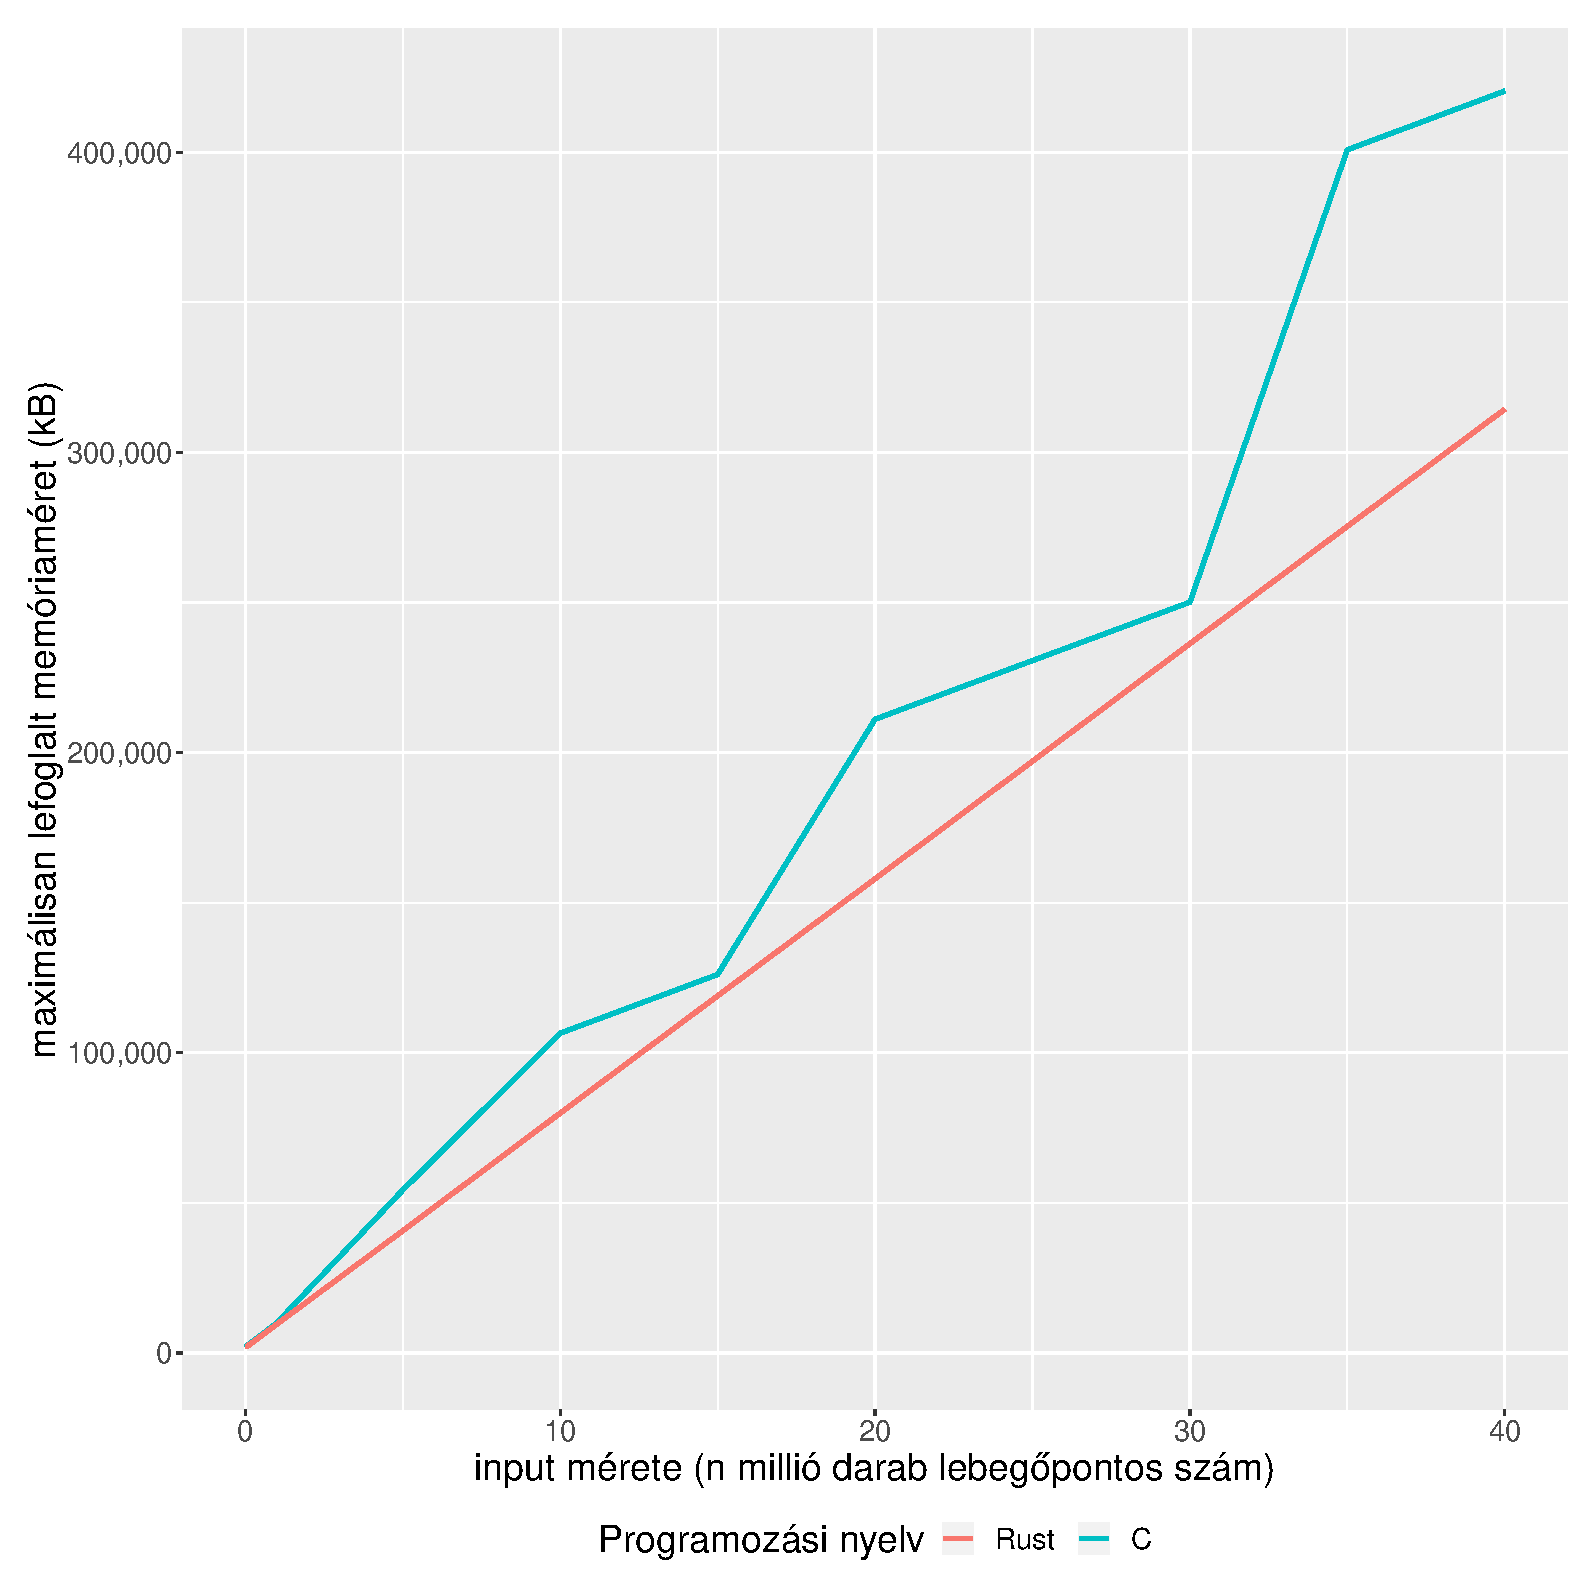
\includegraphics[width=15.5cm]{kepek/linear_interpolation_memory.eps}
A Rust és C nyelven elkészített implementációk között a maximális memóriafoglalást tekintve nincsenek jelentős eltérések.
